\section{Bienvenida}

Cuando accedemos a la aplicación por la ruta principal, veremos la pantalla de bienvenida, a la izquierda tendremos un menú donde podremos registrar un nuevo usuario o bien loguearnos con un usuario ya creado. La aplicación dispone de cuatro perfiles distintos de usuario, cada uno con sus funciones asociadas, estos serían: administrador, planificador, profesor y alumno. Desde esta pantalla solo podremos crear usuarios del perfil alumno y con un e-mail de la UCA válido.\\

\begin{figure}[H] 
  \label{manual-bienvenida} 
	\begin{center}
    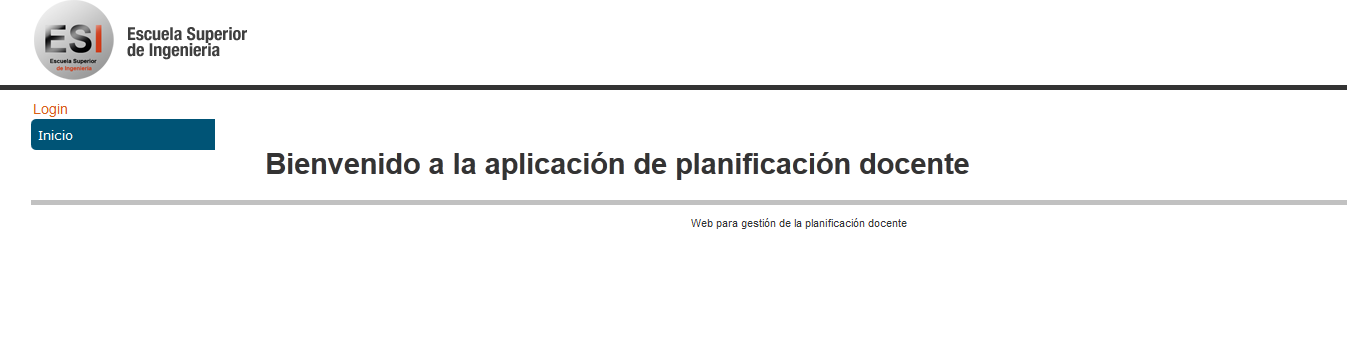
\includegraphics[scale=0.4]{./manual-bienvenida.png}
  \end{center}
\caption{Pantalla de bienvenida de la aplicación}
\end{figure}

El manual está dividido en secciones que detallan las funcionalidades de cada perfil, en primer lugar se explicarán las funciones del perfil administrador, seguido de las de planificador, profesor y alumno.

\section{Perfil administrador}

En primer lugar debemos disponer de un usuario administrador para poder acceder a las funcionalidades de este perfil, para ello, pulsamos sobre el enlace 'login' a la izquierda, y veremos una ventana flotante donde podremos introducir el usuario y contraseña para acceder.\\

\begin{figure}[H] 
  \label{manual-login} 
	\begin{center}
    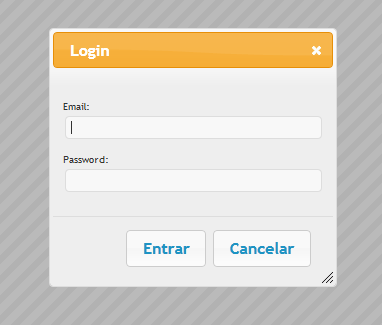
\includegraphics[scale=0.75]{./manual-ventana-login.png}
  \end{center}
\caption{Ventana de login de usuario}
\end{figure}

Una vez dentro, veremos de nuevo la pantalla de bienvenida, pero veremos que en el menú de la izquierda han aparecido nuevas funciones, concretamente los apartados 'Usuario' y 'Configuración'.

\subsection{Administración de usuarios}
\label{manual-administracion-usuarios}

Dentro del apartado usuario podemos hacer diferentes cosas, añadir usuarios, ver los usuarios disponibles en el sistema, editarlos o eliminarlos, incluyendo los datos del propio usuario administrador.

\begin{figure}[H] 
  \label{manual-menu-admin} 
	\begin{center}
    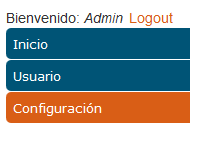
\includegraphics[scale=0.9]{./menu-user-admin.png}
  \end{center}
\caption{Menú lateral con usuario administrador en el sistema}
\end{figure}

\subsubsection{Añadir usuario}
\label{manual-anadir-usuario}
Esta función es exclusiva del perfil administrador y del perfil planificador.\\

Para entrar hacemos click en la opción 'Añadir usuario' dentro del apartado 'Usuario'.\\

A continuación veremos un formulario en el que podremos introducir los datos del usuario a crear asi como el perfil correspondiente a ese usuario, debemos introducir nombre, apellidos y e-mail (es importante que sea un e-mail válido de la UCA, ya que se enviará la contraseña a esa dirección). Una vez pulsemos en enviar, si todos los datos son correctos, se creará el usuario, enviando su contraseña al e-mail dado.

\begin{figure}[H] 
  \label{manual-add-user} 
	\begin{center}
    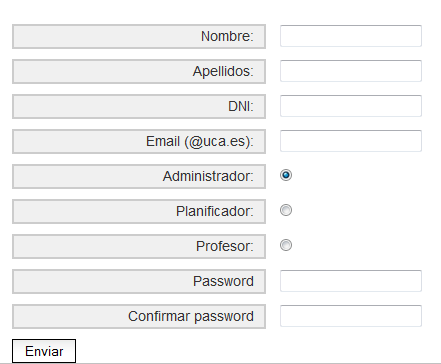
\includegraphics[scale=0.8]{./manual-form-add-user.png}
  \end{center}
\caption{Formulario para añadir un usuario desde el perfil administrador}
\end{figure}

\subsubsection{Ver usuarios}
Esta función es exclusiva del perfil administrador y del perfil planificador.\\

Para entrar hacemos click en la opción 'Ver usuarios' dentro de 'Usuario'.\\

Veremos una lista de todos los usuarios registrados en el sistema, junto a cada uno de ellos tenemos disponible un botón para editar y otro para eliminar el usuario. Si pulsamos sobre editar veremos un formulario similar al del apartado \hyperref[manual-anadir-usuario]{Añadir usuario} pero con los datos del usuario sobreimpresos, podemos modificar los datos que queramos y guardar el usuario, incluído la contraseña.\\

Si pulsamos sobre eliminar, borraremos el usuario del sistema.

\begin{figure}[H] 
  \label{manual-lista-users} 
	\begin{center}
    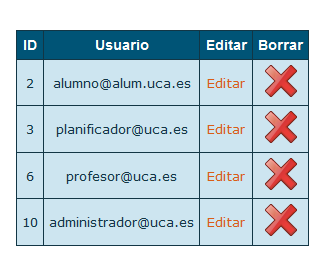
\includegraphics[scale=0.8]{./manual-lista-users.png}
  \end{center}
\caption{Lista de usuarios en 'Ver usuarios'}
\end{figure}

\subsection{Apartado Configuración}

Aquí podremos realizar backups o copias de seguridad de la base de datos de la aplicación, el sistema nos permitirá guardar el archivo .sql resultante. Además podemos restaurar una copia realizada anteriormente, teniendo en cuenta que todos los datos anteriores serán borrados del sistema, por tanto es una función que hay que utilizar con cuidado.

\section{Perfil planificador}
Este es el perfil con más funcionalidad de la aplicación, es donde se controla la funcionalidad principal de la aplicación, es decir la administración y planificación de la carga horaria y docente de las titulaciones de grado. Las funcionalidades que maneja son la creación y edición de titulaciones, asignaturas, cursos, calendario, horarios y planificación docente. Además, al igual que el administrador, también puede crear y editar usuarios.

\subsection{Administración de usuarios}
Esta sección es exactamente igual a la del perfil administrador, para más información consultar \hyperref[manual-administracion-usuarios]{Administración de usuarios}

\subsection{Gestión de titulaciones}
Esta sección es exclusiva del perfil planificador.\\

Desde aquí podemos crear nuevas titulaciones o ver las ya creadas y eliminarlas o editarlas.


\begin{figure}[H] 
  \label{manual-form-add-titu} 
	\begin{center}
    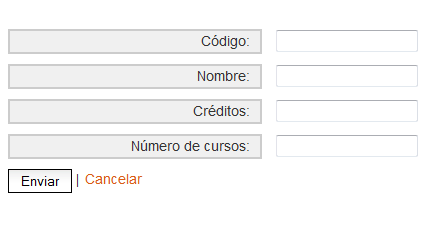
\includegraphics[scale=0.8]{./manual-form-add-titu.png}
  \end{center}
\caption{Formulario para añadir titulaciones al sistema}
\end{figure}

\subsubsection{Añadir titulaciones}
\label{manual-anadir-titulaciones}
Si hacemos click en 'Titulaciones', y a continuación en añadir titulaciones, se nos mostrará un formulario para introducir los datos de una titulación, nombre créditos, y número de cursos que tendrá.

\subsubsection{Editar titulaciones}
Para editar una titulación debemos ir a 'Titulaciones' y a continuación hacer click en 'Ver titulaciones'. Se nos mostrará un listado de las titulaciones disponibles, y tendremos un botón editar a disposición. Si hacemos click en él, veremos un formulario similar al de \hyperref[manual-anadir-titulaciones]{Añadir titulaciones} con los datos de la titulación sobreimpresos pudiendo modificarlos.

\subsubsection{Eliminar titulaciones}
Para eliminar una titulación debemos ir de nuevo al apartado 'Ver titulaciones' y ahí hacer click en el botón de eliminar. Una vez eliminada no podrá recuperarse.

\subsubsection{Ver asignaturas de una titulación}
\label{manual-ver-asignaturas}
Desde el menú ver titulaciones podemos ver las asignaturas de una titulación haciendo click sobre el botón correspondiente.

\subsection{Gestión de asignaturas}
Esta sección es exclusiva del perfil planificador.\\

Desde aquí podremos gestionar todo lo referente a las asignaturas, es decir, listarlas, eliminarlas, editarlas o añadir nuevas. También podemos importar un fichero YML para cargar asignaturas masivamente, cuyo formato se describirá en un anexo aparte.\\

\subsubsection{Añadir asignatura}
Para poder añadir asignaturas debemos listar primero las titulaciones, para ello tenemos un acceso directo en el menú 'Asignaturas'->'Asignatura'. Ahí dispondremos de un botón por cada titulación para poder añadir asignaturas, se nos mostrará un formulario para introducir los datos.

\subsubsection{Resto de operaciones}
Para acceder a ellas debemos ir de nuevo al menú 'Asignaturas'->'Asignatura', y hacer click sobre el enlace 'Ver asignaturas' de una titulación. Esto nos mostrará una lista de las asignaturas con todas las operaciones posibles.

\subsection{Gestión de cursos}
Esta sección es exclusiva del perfil planificador.\\

En el menú cursos tenemos dos accesos, 'Añadir curso', que nos mostrará un formulario para crear un nuevo curso, y 'Ver cursos' desde donde podremos eliminarlos y editarlos.

\subsection{Gestión de aulas}
Esta sección es exclusiva del perfil planificador.\\

Aquí en esta sección, tenemos dos opciones, 'Crear aula' y 'Ver aulas'.

\subsubsection{Crear aula}
\label{manual_crear_aula}
Para crear un aula, hacemos click en la opción 'Crear aula' del menú 'Aulas', esto hará que aparezca un formulario.\\

El formulario está compuesto de dos partes, un campo nombre, para introducir el nombre del aula, y un campo tipos, con varios checkboxes, que podemos marcar. Esto hará que le asignemos actividades posibles que se pueden impartir en ese aula, de forma que cuando estemos creando los horarios, solo podamos asignar un slot de una actividad concreta a un aula que tenga esa actividad asignada. Una vez rellenado el formulario, pulsando en 'Enviar' crearemos el aula.

\subsubsection{Ver aulas}

En esta sección veremos una lista de todas las aulas creadas hasta ahora, pudiendo editar y eliminar cada una. 'Editar' nos mostrará un formulario similar al de \hyperref[manual_crear_aula]{Crear aula}, con los datos asignados sobreimpresos.


\subsection{Gestión de Planificación Docente}

Desde aquí podremos visualizar la planificación docente, crear nuevos planes docentes, o bien importar un csv para hacer cargas masivas de planes docentes de diferentes asignaturas.

\subsubsection{Añadir plan docente}
Al hacer click aquí, se nos mostrará un listado con los cursos disponibles, una vez seleccionemos uno, se nos llevará a otro listado con las titulaciones, y seleccionando una, se nos mostrarán sus asignaturas, a las cuales podremos añadir un plan docente pulsando en el correspondiente enlace. Una vez ahí, se nos mostrará un formulario con una línea por cada actividad, en cada línea una caja para introducir el número de horas totales, otra para las horas semanales y otra para el número de grupos. Además si la actividad no es teoría, se nos mostrará también un checkbox para activar las semanas alternas en esa actividad.
Además tendremos una línea más para añadir los cursos con los que se comparte esa asignatura, en caso de que sea una asignatura común a varias especialidades.\\

Si dejamos alguna caja en blanco, se interpretará como un 0, es decir, si dejamos en blanco la casilla de número de grupos de problemas, significará que habrá 0 grupos de problemas.\\

Si marcamos una casilla de semanas alternas, significará que en la etapa de creación de horarios se asignarán los grupos de dos en dos, es decir, solo veremos la mitad de los grupos que hayamos asignado aquí.

\begin{figure}[H] 
  \label{manual-add-plan} 
	\begin{center}
    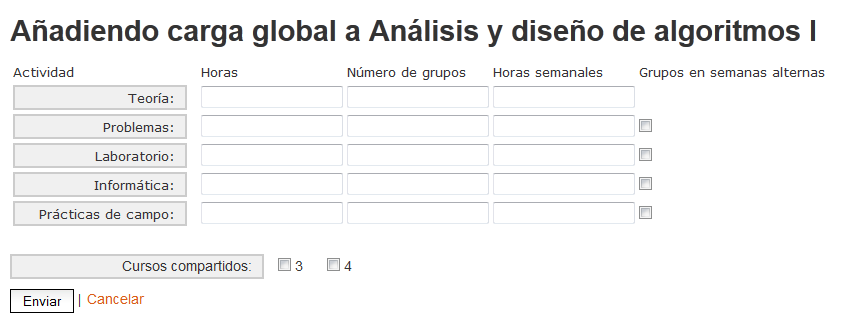
\includegraphics[scale=0.7]{./manual-add-plan.png}
  \end{center}
\caption{Formulario para añadir un plan docente}
\end{figure}

\subsubsection{Importar plan docente}

Desde la opción 'Importar CSV' del menú 'Plan Docente', podemos importar masivamente planes docentes de diferentes asignaturas y titulaciones, tan solo subiendo un archivo con el formato correcto.
El formato necesario se indica en un anexo posterior.

\subsubsection{Ver planificación}

Esta sección funciona de forma similar a la del \hyperref[manual_perfil_profesor]{perfil profesor}, solo que aquí podemos exportar la planificación a un archivo csv, mediante el botón situado en la parte superior izquierda de la pantalla. El formato al que se exporta se expondrá en un anexo posterior.

\begin{figure}[H] 
  \label{manual-visualizacion-plan} 
	\begin{center}
    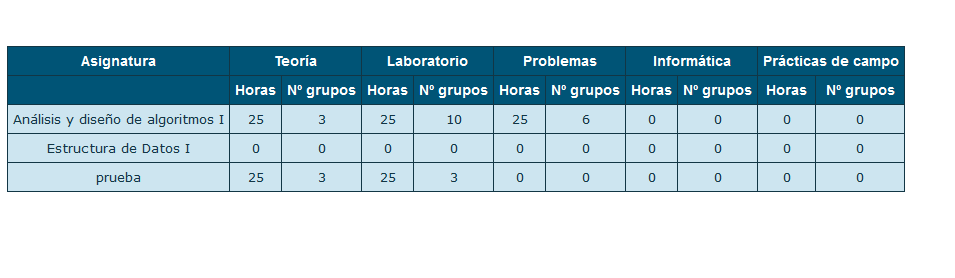
\includegraphics[scale=0.65]{./manual-visualizacion-plan.png}
  \end{center}
\caption{Visualización global de la planificación docente}
\end{figure}

\subsection{Gestión del calendario}

En la opción 'Calendario' en el menú, veremos un calendario en el que podremos añadir eventos al curso actual.\\

La forma de añadir eventos es sencilla, tan solo hay que hacer click sobre una fecha del calendario, se nos mostrará una ventana flotante en la que únicamente tendremos que escribir el nombre del evento que se va a crear.\\

Además también se pueden añadir eventos de más de una fecha, para hacer esto, simplemente tenemos que hacer click sobre una fecha y mantener pulsado el ratón, arrastrando el puntero hasta la fecha de finalización, una vez ahí, se suelta el botón del ratón y se mostrará la ventana para introducir el nombre, se podrá observar que las fechas indicadas son las señaladas.\\

Estas fechas del calendario sirven para hacer el recuento de horas reales impartidas en un curso, esto se explicará en la sección \hyperref[manual_calculo_horas]{cálculo de horas impartidas}.
\\
Además, si queremos borrar un evento ya asignado, únicamente tendremos que hacer click sobre él y nos aparecerá una ventana con dos opciones, 'Borrar' o 'Cancelar', si clickamos en 'Borrar' el evento desaparecerá.

\begin{figure}[H] 
  \label{manual-calendario} 
	\begin{center}
    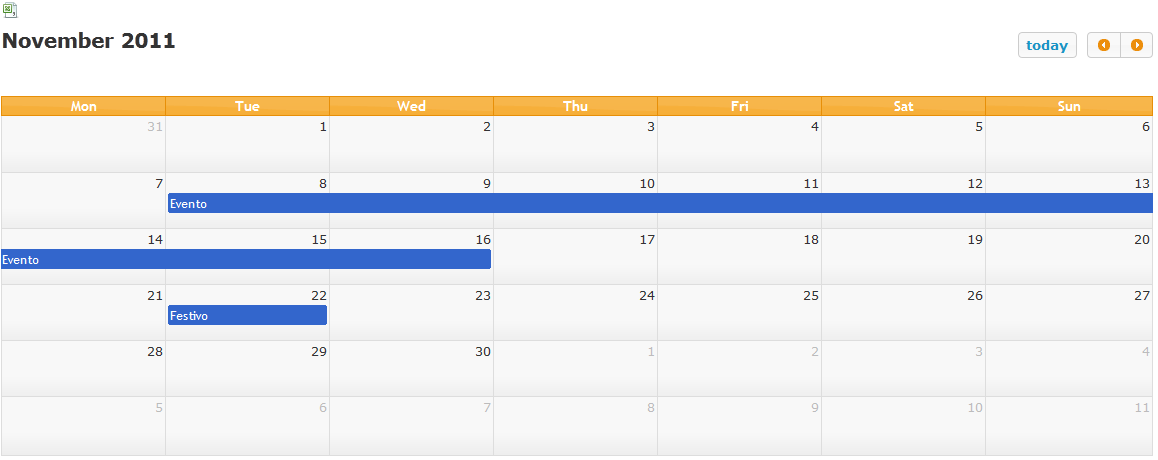
\includegraphics[scale=0.5]{./manual-calendario.png}
  \end{center}
\caption{Visualización del calendario con dos eventos}
\end{figure}


\subsection{Gestión de horarios}
Está sección es también exclusiva de este perfil.
\\
En el menú 'Horarios' solo hay dos opciones, 'Grupos y horarios' e 'Informes de asignatura'.

\subsubsection{Configuración de horarios}

Para configurar los horarios de una titulación, entramos en 'Grupos y horarios', después de seleccionar titulación y curso, veremos una tabla con todos los cursos dentro de esa titulación, a los que podremos añadir grupos o eliminarlos.\\


\begin{figure}[H] 
  \label{manual-seleccion-grupos} 
	\begin{center}
    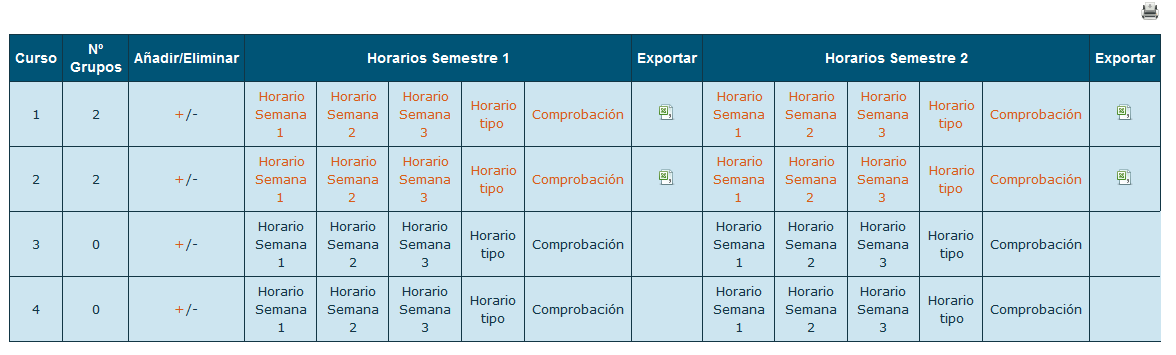
\includegraphics[scale=0.5]{./manual-seleccion-grupos.png}
  \end{center}
\caption{Pantalla de selección de grupos}
\end{figure}

Hay que tener en cuenta que una vez que añadamos un grupo no podremos configurar el horario de asignaturas a las que añadamos planes docentes posteriormente, para ello habría que eliminar el grupo y crearlo de nuevo, por tanto hay que estar seguro de que todas las asignaturas tienen asignada su planifición docente antes de añadir un grupo. Para añadir un grupo pulsamos en el botón '+', esto hará que se creen los horarios para ese curso, tanto del primer como del segundo semestre.\\

El paso inicial es el de configurar el horario tipo, ya que este se copiará a los de las semanas iniciales cuando los editemos, para ello pulsamos sobre el enlace 'Horario tipo' del curso y semestre deseado.
Veremos un cuadro en la parte superior clasificado en pestañas por asignaturas, en cada una de ellas veremos los slots disponibles de cada actividad, con un combo con las aulas disponibles a la que le asignaremos la asignatura, y un color que es con el que aparecerá el slot en el horario. Para asignarlo al horario simplemente tenemos que hacer click sobre el slot, manteniendo pulsado y arrastrarlo al horario en la parte inferior, colocándolo en el lugar deseado. Si hay algún problema, por ejemplo que el aula esté ocupada, o que el grupo se pise con otro y no esté permitido, el slot volverá a su lugar en la parte superior y no se asignará al horario.\\

\begin{figure}[H] 
  \label{manual-configuracion-horario} 
	\begin{center}
    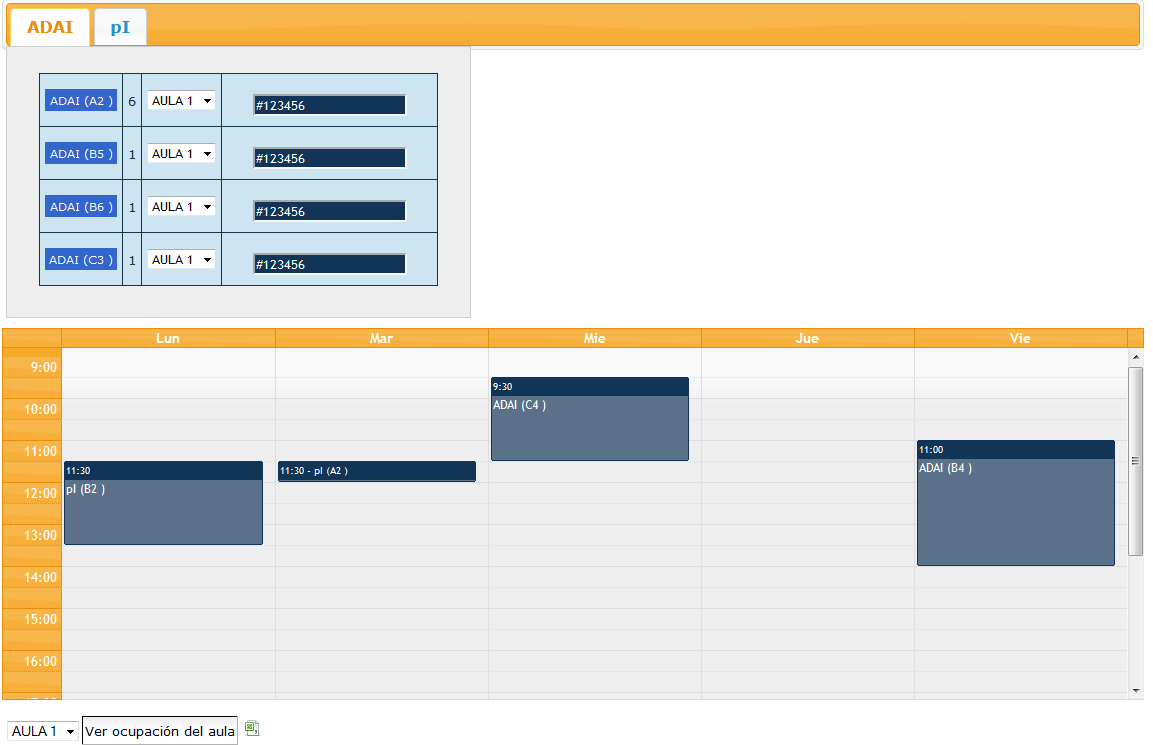
\includegraphics[scale=0.5]{./manual-configuracion-horario.png}
  \end{center}
\caption{Pantalla de configuración de horarios}
\end{figure}

Una vez asignado un slot, podemos moverlo sin problemas a otro lugar en el horario, o incluso borrarlo, para ello, simplemente hacemos click sobre el slot, y a continuación hacemos otro click en el botón borrar, esto hará que el slot vuelva al cuadro superior, pudiéndolo asignar de nuevo si lo deseamos.\\

Otra posibilidad es visualizar la ocupación de un aula concreta, para ello la seleccionamos en el combo correspondiente y hacemos click en 'Ver ocupación de aula' en la parte inferior. Esta ocupación la podemos exportar haciendo click en el botón con el icono de CSV junto al de 'Ver ocupación de aula'.
\\
Podemos ir directamente a un horario de las semanas iniciales con los botones de la parte superior, el funcionamiento para editar estos horarios es exactamente el mismo, solo que no veremos los grupos que no sean de teoría.

\subsubsection{Exportar horarios}

Para exportar un horario a CSV debemos ir al menú 'Grupos y horarios', y en la columna exportar pulsar sobre el botón correspondiente, esto exportará todos los horarios de ese semestre para esa titulación y curso, es decir, tanto semanas iniciales como horario tipo.

\subsubsection{Comprobación de horas impartidas}

Una vez configurados los horarios, en el menú 'Grupos y horarios' tenemos una columna con el botón 'Comprobación', que nos mostrará una tabla con las horas planificadas y las que se impartirán realmente según la configuración de los horarios, de forma que si faltan horas cambiemos lo que sea necesario.  

\subsubsection{Informes de asignatura}
En el menú 'Informes de asignatura' podremos realizar informes detallados de las horas de las asignaturas que deseemos, estos informes se exportarán a PDF, e incluirán las asignaturas que seleccionemos en la pantalla correspondiente. En el informe se verán las horas impartidas por cada semana, actividad y grupo.

\begin{figure}[H] 
  \label{manual-informe} 
	\begin{center}
    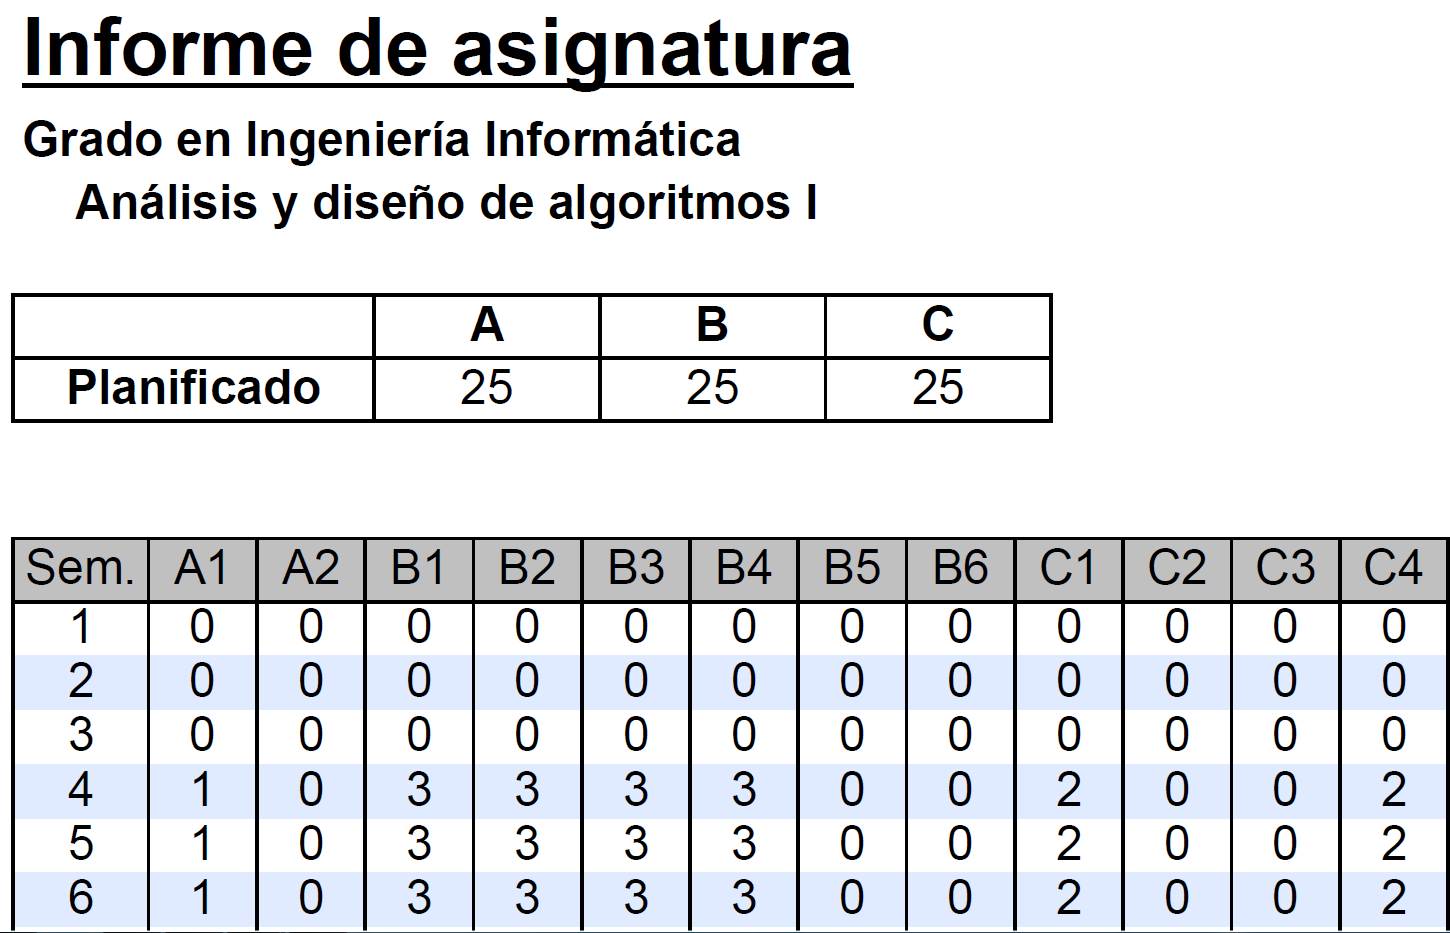
\includegraphics[scale=0.3]{./manual-informe.png}
  \end{center}
\caption{Parte de un informe de una asignatura}
\end{figure}

\section{Perfil profesor}
\label{manual_perfil_profesor}
El perfil profesor solo tiene una finalidad, que es el de la visualización de la planificación global para un curso de las titulaciones, la visualización se hace a través de las titulaciones, y no desde una asignatura como si puede hacer el planificador.\\

Para ello, el profesor selecciona 'Planificación Docente' en el menú de la izquierda y a continuación la opción 'Ver planificación', que es la única disponible. Al usuario se le pedirá seleccionar un curso, y a continuación, una titulación. Se visualizará entonces una tabla con la planificación docente de todas las asignaturas de esa titulación, clasificado por actividad.\\

Además de esto, el profesor, al igual que todos los demás usuarios, puede cambiar su contraseña.
\\
Ver figura~\ref{manual-visualizacion-plan} en la página~\pageref{manual-visualizacion-plan}.

\section{Perfil alumno}

El perfil alumno solo tiene una opción, que es la de la visualización de horarios.\\

El alumno es un tipo de usuario especial, tiene una titulación asignada, por tanto no deberá seleccionar la titulación de la que quiere ver el horario, sino que automáticamente serán visibles solo las asignaturas de su grado.\\


\begin{figure}[H] 
  \label{manual-alumno-seleccion} 
	\begin{center}
    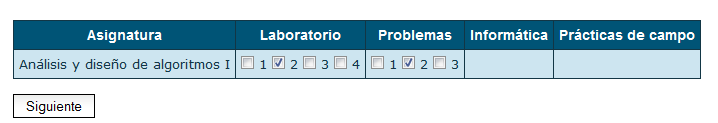
\includegraphics[scale=0.7]{./alumno-seleccion-grupos.png}
  \end{center}
\caption{Selección de un alumno de los grupos para visualizar un horario}
\end{figure}

Para proceder a la personalización del horario, el alumno debe seleccionar 'Horarios' en el menú de la izquierda, y a continuación 'Ver horario'. Después de seleccionar el curso de la lista ofrecida, aparecerá un listado de las asignaturas disponibles, se podrán seleccionar las deseadas y el grupo de teoría que se quiere visualizar. Una vez seleccionado, en el paso siguiente se ofrecerá un listado de las asignaturas anteriormente seleccionadas junto con sus actividades y grupos, pudiendo seleccionar los que se quieran para configurar un horario a medida.\\

Una vez configurado veremos los horarios de las primeras semanas y el horario tipo de las asignaturas seleccionadas.
